\renewcommand{\sectionautorefname}{Section}
\let\subsectionautorefname\sectionautorefname
\let\subsubsectionautorefname\sectionautorefname
\section{Method}
\label{sec:method}



%%%%%%%%%%%%
\begin{comment}
\subsection{Implementation overview}
\label{sec:imploverview}

An agent will be modeled in \gls{ttr} and implemented in PyTTR.
The purpose of the agent is to perceive a scene, parse a question related to the scene and answer it.

The agent will receive a 2D image as well as a natural-language question as input.
Perceptual processes are performed on the image, which results in a set of beliefs.
The question is parsed and evaluated against the beliefs in order to obtain an answer.

While operational functionality and the overall procedural code is written in Python, the core model is written in \gls{ttr} (realized as Python code using PyTTR).
As such, \gls{ttr} serves as a formal specification language.
This additional layer provides formal transparency and type robustness.
% What?

This section will describe some tools and frameworks used to formulate and implement the model.
\end{comment}
%%%%%%%%%%%%%%



\subsection{PyTTR: Programming with \gls{ttr}}
\label{sec:pyttr}

\cite{pyttr} provides a Python implementation of \gls{ttr} known as PyTTR.
It supports the modeling of \gls{ttr} types and operations such as judgement and type checking.
As a Python library it also enables other features and peripheral procedures to be written in Python.

PyTTR allows, in turn, the implementation of \gls{ttr} models.
By implementing a theoretical model as a computer program, it can ``come alive'' and be tested on real problems and data.
When implemented, the model can be evaluated and compared in practical settings to other models.

%[What has been written in PyTTR so far? nu, animat]



\subsection{Object detection with YOLO}

\textbf{You only look once (YOLO)} \citep{RedmonYouOnlyLook2015} is a neural network model for image recognition.
Given an image, it will detect objects and classify them.
Each detection consists of a bounding box in pixel coordinates, a class label and a confidence score between 0 and 1.

YOLO is trained using a loss function which takes detection as well as classification into account.
In other words, it simultaneously predicts bounding boxes and classifies the contained objects.
Unlike \cite{HeMaskRCNN2017} and others, it does not contain any recurrent layers.
The joint, recurrence-free model makes for a rather small network size and a high evaluation speed, although it does lag behind in accuracy compared to the state of the art \citep{RedmonYouOnlyLook2015}.

The model exists in a few different network configurations, which have all been trained on the COCO dataset \citep{LinMicrosoftCOCOCommon2014}.
Development within this thesis has been using the ``YOLOv2'' configuration \citep{redmon_yolo_2018}.


\begin{figure}[h]
\label{fig:dogbike_annotated}
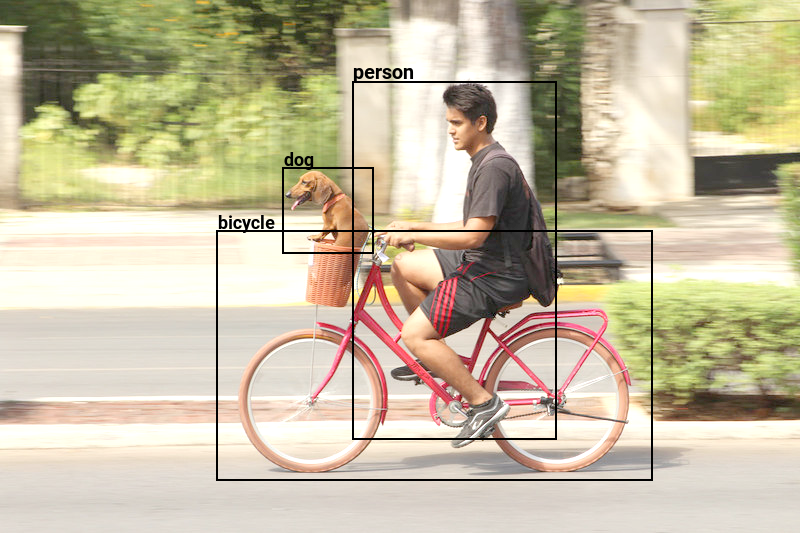
\includegraphics[width=\textwidth]{dogbike_annotated}
\centering
\caption{Visualization of the labels and bounding boxes emitted by YOLO when given an image depicting a cyclist with a dog.}
\end{figure}

YOLO is written in C, using the Darknet neural network library \citep{darknet13}.
It can be used in Python with the TensorFlow machine learning library \citep{tensorflow2015-whitepaper} and the Darkflow library \citep{trieu_darkflow_2018} which translates a Darknet model to TensorFlow.

When invoked from Python, the return value is a collection of dictionary objects, each containing a label, coordinates and a confidence score, as exemplified in \autoref{lst:yoloout}.
Results with confidence over a certain threshold are cast into \gls{ttr} records.
In this process, the bounding box coordinates are cast from a top-left and bottom-right tuple $\langle\langle x_1, y_1\rangle, \langle x_2, y_2\rangle\rangle$ to a center-width-height tuple $\langle x_c, y_c, w, h\rangle$ (later defined as the $Segment$ type), as the latter is more adequate for the spatial classification used in this project.

\begin{lstlisting}[label=lst:yoloout, caption=Example output of YOLO invocation]
[
    {
        'topleft': {'x': 354, 'y': 86},
        'bottomright': {'x': 551, 'y': 437},
        'label': 'person',
        'confidence': 0.80116189,
    },
    {
        'topleft': {'x': 224, 'y': 234},
        'bottomright': {'x': 646, 'y': 476},
        'label': 'bicycle',
        'confidence': 0.85828924,
    },
	...
]
\end{lstlisting}



\subsection{Objects and perception with \gls{ttr}}

The perception of objects in this model is largely based on \citet[Section 5.1]{lspc}.
First, the object detection algorithm returns a set of \textit{perceptual objects}.
Each of these is evidence that a certain location is associated with a certain property (such as being a dog).
%It does not, however, constrain any individual to this association.
Second, an \textit{individuated object} is generated for each perceptual object.
The individuated object additionally refers to a specific individual, and explicitly associates the property and the location with this individual.
%This describes the situation that there is an individual, which has the given property, at the given location.
%In the \gls{ttr} implementation (presented in full in \autoref{sec:ttrmodel}), the individuated object is a type.
%[what's so good about it being a type?] \cite{BarwiseSituationsAttitudes1981}
%While the perceptual object only couples a property together with a location, the individuated object is the type of situations where, for example, the individual $a_1$ is a dog at location $l_1$.
It is the type of situations where, for example, the individual $a_1$ is a dog at location $l_1$.

In \cite{lspc}, the world has the form of a 3D point space rather than a 2D image.
This necessitates different types for the perceptual input and the locations of perceived objects.
In the point space case, the $PointMap$ list type (a list of points) is used for the full ``world''.
Any part of the world is also a list of points, thus also a $PointMap$.
In our case, $Image$ is used for the full image but we use $Segment$ to refer to parts of it.



\subsection{Spatial relations}
\label{sec:method-spatrel}
% Classification algorithm non-TTR. Simplistic, compare to sophisitcated alternatives.

Our method of spatial relation classification is inspired by \cite{ttrspat} but more simplistic.
One simplification is that the reference frame is fixed.
In the words of \cite{Garnhamunifiedtheorymeaning1989}, this means we only consider the deictic meaning of spatial relation terms, and not the intrinsic.
``Left'' will mean to the left in the plane of the image, even if the reference object is turned on the side or toward the viewer.
Another simplification is the neglection of the \textit{functional} aspects of spatial relations \citep{CoventryInterplayGeometryFunction2001}.

In our model, a spatial classifier $\kappa$ takes two locations and returns a boolean result.
We have implemented spatial classifiers as Python functions.
For the purpose of this thesis, no sophisticated spatial classification has been considered.
Instead, a naive comparison between centers of bounding boxes was implemented using pre-defined rules.
This was done for the four relations ``left'', ``right'', ``above'' and ``below''.



\subsection{Language and \gls{vqa}}
\label{sec:languagevqa}

In contrast to full \gls{vqa} systems, the model presented in this thesis will be restricted to a limited type of questions, namely polar questions on the location of one object in relation to another.
Such a question has a corresponding declarative statement:
The question ``Can you see them?'' corresponds to the statement ``You can see them''.
% TODO source?

Giving the natural-language utterance a representation in the same formal framework as the image allows comparing them to each other.
% TODO Comparing?
The system will laborate with a \textit{question type} ($Q$) representing the question, as well as a \textit{scene type} ($S$) representing the perceived scene.

The situation described by the question type will be true if there exists a witness of that type, $r:Q$ \citep{BarwiseSituationsAttitudes1981,CooperAustiniantruthattitudes2005}.
The scene type, on the other hand, is considered true by virtue of being generated by perceptual classification.
It follows that the question type is true if it is a supertype of the scene type.
Thus, rather than looking for a witness to the question type, we formulate the problem as subtype checking, described in detail in \autoref{sec:subtyperelabeling}.
%However, the subtype relation requires matching field labels, which will not be the case here, as labels are generated on the fly.
%Thus, the condition is reformulated to allow relabeling \citep[pp. 133–135]{CooperTypetheorylanguage2016}:
The question is answered with ``yes'' or ``no'' depending on whether the scene type is a subtype of the question type, $S \sqsubseteq Q$.

The existing research on \gls{ttr}-based approaches to natural-language parsing, overviewed in \autoref{sec:ttnlp}, might be extensive enough to cover the kind of utterances considered here.
However, there is currently no implementation available and ready to use, and parsing is not within the main focus of this thesis.
Therefore, the natural-language parsing implemented for this thesis is instead a simplistic one, detailed in \autoref{sec:parsing}
%It uses feature structure context-free grammar (FCFG) tools available in NLTK \citep{BirdNaturalLanguageProcessing2009} to parse text into \gls{fol} expressions.
%With a custom function, the \gls{fol} expressions are transformed to a TTR record type.
%As an example, the question ``Is there a dog to the left of a car?'' is parsed into the type in \autoref{eq:uttex}.

%\begin{equation}\label{eq:uttex}
%\left[\begin{array}{rcl}
%\text{x} &:& Ind\\
%\text{y} &:& Ind\\
%\text{c}_\text{dog} &:& \text{dog}(x)\\
%\text{c}_\text{car} &:& \text{car}(y)\\
%\text{c}_\text{left} &:& \text{left}(x, y)\\
%\end{array}\right]\end{equation}

%[classification before/after question]
